\section{Crypt$\epsilon$ Primitives}
\subsection{Primitive Definitions} 
The input to Crypt$\epsilon$ is an encrypted instance of a database $\boldsymbol{\tilde{\mathcal{D}}}$ with a single relational schema $\langle \mathcal{A}_1,\mathcal{A}_2, . . . ,\mathcal{A}_l\rangle$. Each attribute $\mathcal{A}_i$ is assumed to be discrete
(or suitably discretized) and represented in one-hot-coding form. 
There are two types of Crypt$\epsilon$ primitives namely transformations and measurement.
\subsubsection{\textbf{Transformation}}
 Transformation primitives take
as input an encrypted data source variable (a table of size $x \times y, x,y \in \mathcal{Z}_{\geq 0}$) and output
a transformed data source (again  a table $x' \times y', x',y' \in \mathcal{Z}_{\geq 0}$) that is still encrypted. Typically $x$ and $x'$ are equal to $m$, the total number of data owners, i.e., every tuple in the data source tables corresponds to the record of a single data owner. In case $x=1$ or $x'=1$ the data source is an encrypted vector and we represent it as $\mathbf{V}$.
The transformation primitives are mostly carried out by the \textsf{AS} on its own; this is enabled by our use of labeled homomorphic encryption scheme which allows us to perform certain operations, specifically multiplication and addition, directly over the encrypted data. %Only two transformations  (\textsf{GroupBy} and \textsf{CountDistinct}) need to be computed via a secure computation protocol between the \textsf{AS} and the \textsf{CSP}. 
Since these primitives work entirely on encrypted data, they do not expend the privacy budget. However these operators can affect the privacy analysis through their stability. Every transformation in Crypt$\epsilon$ has a well-established stability.
For each record of the database $\boldsymbol{\tilde{\mathcal{D}}}$ (i.e., data corresponding to a single data owner) we maintain an encrypted bit which indicates whether the record is relevant to the program at hand. Let $\mathbf{B}$ represent this bit vector where $\mathbf{B}[i]$ corresponds to this indicator bit for the $i^{th}$ record.  If $\mathbf{B}[i] =Enc_{pk}(1)$, then the $i^{th}$ record is to be considered for answering the current program and vice versa. Only one of the transformation, \textsf{Filter} alters the bit vector $\mathbf{B}$. Before every program execution, $\mathbf{B}$ is initialized to a 1-vector. 
\begin{enumerate}

	\item \textsf{CrossProduct} ($\tilde{\mathbf{T}}, A_i, A_j$) - Given encrypted one-hot-codings for two different attributes $A_1$ and $A_2$ of domain sizes $s_{A_1}$ and $s_{A_2}$ respectively, the goal of this transformation is to compute the encrypted one-hot-coding for the entire two-dimension domain of the new $\lq$attribute' $A_1\times A_2$ of size $s_{A_1}\cdot s_{A_2}$. Thus this transformation takes as input a $x \times y $ table, $\tilde{\mathbf{T}}$ defined over attribute set $A=\{A_1,A_2,...,A_y\}$ where each cell $\tilde{\mathbf{T}}[i,j] , i \in [x], j \in [y], 2 \leq y \leq k$ corresponds to the encrypted one-hot-coding for attribute $A_j$ for the data owner $\textsf{DO}_i$ and outputs a $x \times (y-1)$ table with attribute set $\{A_1\times A_2,A_3,\ldots,A_{y}\}$.  Note that the construction of the one-hot-coding of the full $y$-dimension domain can be computed by repeated application of this transform. 	
    
	
	\item \textsf{Project}($\tilde{\mathbf{T}},A^*$)- In addition to the $ x \times y$ table, $\tilde{\mathbf{T}}$ over attribute set $\{A_1, A_2, ..., A_y\}$, the \textsf{Project} transformation takes a set of attributes $A*=\{A^*_1,...A^*_p\}, p < y$ as inputs. The result of the transformation is defined as the $x \times p$ data source table where each record is just restricted to the attribute set $A^*$, i.e., it discards all other attributes. 
	%Infact it is analogous to the operation of marginalization which is described as follows.
	%Assuming  $A$ and $B$ to be two attributes with finite domains, let $x$ be a vector of counts representing a histogram over the cross product of the domain (with $|A|*|B|$ entries).
	%Marginalization over the attribute $B$ results in a vector of counts on the attribute $A$ alone by adding up counts corresponding to the same value of $A$.  
   
  \item \textsf{Filter}($\tilde{\mathbf{T}},\phi$) - Let $\tilde{\mathbf{T}}$ be an encrypted table of one-hot-codings over attribute set $A=\{A_1,...,A_k\}$, $\phi$ be a  predicate defined over a subset of attributes $A^*\subseteq A$ and $\mathbf{B}$ be the current state of the indicator vector which is stored by the \textsf{AS}. The predicate $\phi$ has to be expressed as a conjunction of range conditions over $A^*$, i.e.,\begin{gather}\phi = \bigwedge_{A \in A^*}(A \in \{v_{1},\ldots,v_{t}\} ) \label{phi} \end{gather} If for some attribute $A \in A^*$, the condition is a equality condition as $A==v$ instead of a range condition, then simply put $v_1=v_t$. For e.g., a condition of this form is find the number of records that satisfy $Age$ in range [30,40] and $Gender$ is male. For each record $r_i, i \in [m]$, the Filter transformation zeros the corresponding indicator bit $\mathbf{B}[i] $ if $\phi(r_i)=False$. $\mathbf{B}[i] $ is kept unchanged otherwise. Thus the \textsf{Filter} transformation suppresses all the records that are extraneous to answering the program at hand (i.e., does not satisfy $\phi$) by explicitly zeroing the corresponding indicator bits and outputs the updated indicator vector. %It takes as input a $x \times 1$ table $\tilde{\mathbf{T}}$, whose every row is an encrypted one-hot-encoding (of the form $\mathbf{\tilde{R}}$) for the attribute of concern $A$, and a vector $\mathbf{C}$ which has encryptions of appropriate non-zero weights for indices that satisfy $\phi$. %Note that $A$ need not be an attribute of the original attribute set $\mathcal{A}$ but can be a new multi-dimension 'attribute' constructed over $\mathcal{A}^* \subseteq \mathcal{A}$, i.e., $A= \prod_{A*_i \in \mathcal{A}^*  }A^*_i$. 
    \item{\textsf{Count}($\mathbf{T}$) } - The \textsf{Count} transformation outputs the encrypted value of the non-noisy true count for the program at hand. For answering linear counting queries, typically \textsf{Count}  is the last transformation to be applied and is immediately preceded by a \textsf{Filter} transformation. Recall that the \textsf{Filter} transformation sets bit $i \in [m]$ to be 1 (encrypted) if the $i^{th}$ record satisfies the filter condition and 0 otherwise and outputs this encrypted $m\times 1$ vector. Hence the \textsf{Count} primitive simply adds up all the entries of this bit vector $\mathbf{B}$ and  outputs the sum which is a single encrypted value. 
    \item{\textsf{GroupBy*}($\mathbf{\tilde{T}},A$)}- The purpose of the \textsf{GroupBy*} transformation is to essentially bucket the input $x\times y$ table $\mathbf{\tilde{T}}$ into groups of records having the same value for an attribute of choice $A$. The output of this transformation is an $1\times s_A$ encrypted  vector $\mathbf{V}$  where each vector element $\mathbf{V}[i], i \in [s_A]$ represents the encrypted count of the number of records in $\boldsymbol{\tilde{\mathcal{D}}}$ having value $v_{i}$ for attribute $A$. Thus \textsf{GroupBy*} essentially returns an encrypted histogram for $A$.
    This primitive serves as a preceding transformation for other Crypt$\epsilon$ primitives like \textsf{NoisyMax}, \textsf{CountDistinct} et al.
     \item{\textsf{GroupBy}($\mathbf{\tilde{T}},A$)-} The \textsf{GroupBy} transformation is similar to the aforementioned \textsf{GroupBy*} transformation. The only difference between the two is that, the former outputs the encrypted one-hot-coding of the respective counts. That is, the output of \textsf{GroupBy}($A$)  is an $s_A$ lengthed encrypted vector $\tilde{\mathbf{V}}$ such that each element, $\tilde{\mathbf{V}}[i], i \in [s_A]$ represents the encrypted one-hot-encoding of the number of records in $\boldsymbol{\tilde{\mathcal{D}}}$ having value $v_{i}$ for attribuet $A$. This transformation allows us to answer queries based on the count of a particular value for attribute $A$.
     %Note that since for \textsf{GroupBy} we need to create the one-hot-coding of the counts, this requires an interaction with the \textsf{CSP}.
     \item {\textsf{CountDistinct}($\mathbf{V}$)-} As mentioned before, the \textsf{CountDistinct} primitive takes as input an encrypted vector $\mathbf{V}$ which is the output of a \textsf{GroupBy*}($A$) primitive for some attribute $A$. Thus the \textsf{CountDistinct} primitive  returns the number of distinct values of $A$ that appear in the records of $\boldsymbol{\tilde{\mathcal{D}}}$ by counting the non-zero entries of $V$.  
\end{enumerate}
%Note that the first four transformations namely \textsf{CrossProduct, Project, Filter} and Count are performed by the \textsf{AS} alone. Only for transformation \textsf{GroupBy} the \textsf{AS} engages in a secure computation protocol with the \textsf{CSP}.
\subsubsection{Measurement} The measurement operators involve implementing the differentially private algorithms of laplace mechanism and noisy max.  Thus they expend the privacy budget and require secure computation between the \textsf{AS} and the \textsf{CSP}. 
\begin{comment} All measurement operators must involve joint computation with the \textsf{CSP}. Note that the requisite noise to be added to ensure differentially privacy has to be jointly added by both the \textsf{AS} and the \textsf{CSP}. It is so because, had only either one of the servers added the noise, then that server would be able to retrieve the true non-noisy answer by simply de-noising the published differentially private answer. This means that the sensitivity of the program being executed should be known to both the servers. This poses no hindrance in our setting  since the program is public, the  sensitivity computation can be performed very easily by observing the sequence of the preceding transformations.
\end{comment}
\begin{enumerate}
	\item \textsf{Laplace}($\mathbf{V},\epsilon$) - In the Laplace mechanism, in order
to publish $f(D)$ where $f : D \mapsto R$, $\epsilon$-differentially private mechanism $\mathcal{M()}$ 
publishes $f(D) + Lap\Big(\frac{\Delta f}{\epsilon}\Big)$  
where $\Delta f = \max_{D,D'}||f(D)-f(D')||_1$ is known as the sensitivity of the query. The p.d.f of $Lap(b)$ is given by\begin{gather}\mathbf{f}(x)={\frac  {1}{2b}}e^{ \left(-{\frac  {|x-\mu |}{b}}\right)}\end{gather} The sensitivity of the function $f$ basically captures the magnitude by which a single individual's data can change the function $f$ in the worst case. Therefore, intuitively, it captures the uncertainty in the response that we must introduce in order to hide the participation of a single individual. For counting queries the sensitivity is 1. The \textsf{Laplace} primitive enables the \textsf{AS} and the \textsf{CSP} to add two separate instances of random laplace noise to the true result of a counting query for generating a differentially private output. It takes an input an encrypted vector $\mathbf{V}$ (could be a scalar too) and adds two instances of noise drawn from $[Lap(\frac{1}{\epsilon})]^{|V|}$ to it.

	\item \textsf{NoisyMax}($\mathbf{V},\epsilon, k$)-Noisy-Max is a type of differentially-private selection mechanism where the goal is to determine the counting query with the highest value out of $n$ different counts.  
	The algorithm works as follows. First, generate each of the counts and then add independent Laplace noise from the distribution $Lap(\frac{1}{\epsilon})$ to each of them. The index of the largest noisy count is then reported as the noisy max.
	This has two fold advantage over the naive implementation of finding the maximum count.
Firstly, noisy-max applies "information minimization" as rather than releasing all the noisy counts
and allowing the analyst to find the max and its index, only the
index corresponding to the maximum is made public.
Secondly, the noise added is much smaller than that in the case of the naive implementation (it has sensitivity $\Delta f=m$). Thus the \textsf{NoisyMax} primitive takes as input of encrypted vector where each vector element is a count. It then adds noise drawn from $Lap(\frac{1}{\epsilon})$ to each vector element and computes the indices of the top k elements.
\end{enumerate}
%To demonstrate the use of Crypt$\epsilon$ primitives let us look at the following example.
\subsection{Implementations}\label{implementation}
In this section we describe the implementation of Crypt$\epsilon$. First we discuss our proposed technique for extending the $labMult()$ operation of \textsf{labHE} to support $n > 0$ multiplicands.  
 \paragraph*{\textbf{General n-way multiplication for \textsf{labHE}- $genLabMult()$}}
Consider the case where we want to multiply the respective ciphers of  $n$ messages $\{m_1,...m_n\} \in \mathcal{M}^n$. Note that the reason why we can't simply use $labMult$ for a generic $n-$ way multiplication is because, the "multiplication" cipher $\mathbf{d}=labMult(\mathbf{c_1},\mathbf{c_2})$ does not have  a corresponding label. Thus for generalizing the $labMult()$ operation for $n$ multiplicands what we have to do is to generate a label and a seed for every intermediary product of two multiplicands. This can be done in the following way-  \\
Consider two ciphers $\mathbf{c_1}$ and $\mathbf{c_2}$ corresponding to messages $m_1$ and $m_2$. The \textsf{AS} computes 
$\textbf{d}'=labMult(\mathbf{c_1,c_2}) \oplus Enc_{pk}(r)$ where $r$ is a random mask such that $Dec_{sk}(\textbf{d}')=m_1\cdot m_2-b_1\cdot b_2+r$. The \textsf{AS} sends $\textbf{d}'$ to the \textsf{CSP}. Now the \textsf{CSP} decrypts it and removes  $b_1\cdot b_2$ to get plaintext $d'=m_1\cdot m_2+r$. Note that the mask $r$ protects the value of $m_1\cdot m_2$ from the \textsf{CSP}. The \textsf{CSP} next assigns a seed $\sigma'$ and label $\tau'$ to the product and returns the value $\bar{c}=(\bar{a},c')$ to the \textsf{AS} where $\bar{a}=m_1\cdot m_2 -b' +r$, $b'=\mathcal{F}(\sigma',\tau')$ and $c'=Enc_{pk}(b')$ to the \textsf{AS}. The \textsf{AS} can subtract $r$ from $\bar{a}$ to obtain the  true value of the hidden message $a'=m_1\cdot m_2 - b'$. However since $b'$ is not known to the \textsf{AS}, $m_1\cdot m_2$ remains hidden from the \textsf{AS} as well. Now with the true cipher $\mathbf{c}=(a',c')$ for the product the \textsf{AS} can compute further multiplications on it. 
For a generic $n-way$ multiplication the order of multiplication can be, in fact, parallelized as  shown in Figure 2 to require a total of $\lceil \log n\rceil$ rounds of communication with the \textsf{CSP}. 
\begin{figure}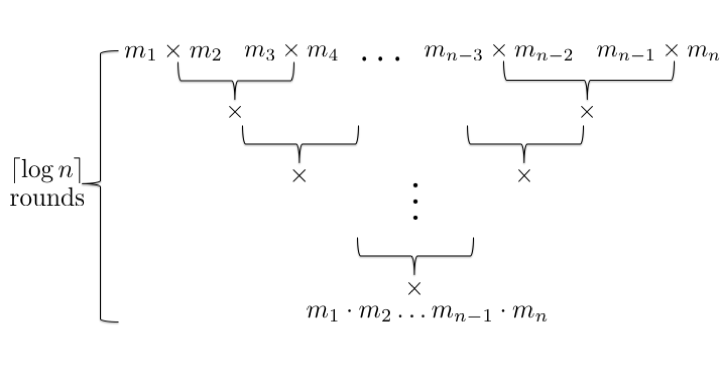
\includegraphics[height=4cm,width=8cm]{kk.png} \caption{ $genLabMult()$ - Batching of multiplicands for \textsf{labHE}} \end{figure}\\
Now let us explain the implementation details of the aforementioned Crypt$\epsilon$ primitives. 
\begin{enumerate}\item \textsf{CrossProduct}($\tilde{\mathbf{T}}, A_i, A_j$): Let $D_1$ and $D_2$  be the encrypted one-hot-coding corresponding to two  values $v_1$ and $v_2$ (integral representation) for attributes $A_1$ and $A_2$ respectively. The corresponding encrypted one-hot-encoding for the two-dimensional attribute $A_1\times A_2$ is given by  \begin{gather} D_{1\times 2}[(i-1)\cdot s_{A_2}+j] = labMult(D_1[i], D_2[j])\\ i \in [s_{A_1}], j \in [s_{A_2}]\end{gather} For this particular case, only $D_{1 \times 2}[(v_1-1)\cdot s_{A_2}+v_2]=Enc(1)$ while all other indices will equate to $Enc(0)$. Note that when computing the one-hot-encoding for a t-dimensional attribute $t > 2$,  for the actual implementation, instead of calling $t$ iterative instances of \textsf{CrossProduct}() we use the $genLabMult()$ operator of labeled homomorphic encryption to speed up the computation. \item \textsf{Project}($\tilde{\mathbf{T}}, A^*$)- The implementation of the \textsf{Project} transformation is very straightforward, it simply drops off all the attributes from $\tilde{\mathbf{T}}$ and returns the truncated table. \item \textsf{Filter}($\mathbf{\tilde{T}},\phi$)-  As discussed in the preceding section, the predicate $\phi$ is expressed in a special form of conjunctions of range conditions given by eq \ref{phi}. Now for a range condition $A \in \{v_1,...v_t\}$, assuming $\mathbf{\tilde{R}_A}[i]$ is the corresponding one-hot-coding for the $i^{th}$ record's value for attribute $A$,  consider the following \begin{gather}\mathbf{c}_A^i=\bigoplus_{j=1}^{t}\tilde{\mathbf{R}}_{A}[i][v_1]\end{gather} where $\tilde{\mathbf{R}}_{A}[i][v]$ is the $v^{th}$ index of corresponding one-hot-coding. Clearly if the $i^{th}$ record satisfies the condition $A \in \{v_1,...v_t\}$, then exactly one of the values in $\{\tilde{\mathbf{R}}_{A}[i][v_j]\}, j \in \{1,...,t\}$ will be a cipher for $1$. Thus $c_A^i=1$ if record $i$ satisfies the range condition and 0 otherwise. If the condition is instead an equality predicate $A==v$ then $\mathbf{c}_A^i=\tilde{\mathbf{R}}_{A}[i][v]$. Now considering $\phi$ is given by eq \ref{phi}, let us define\begin{gather}\mathbf{c}^i=genLabMult(\mathbf{c}^i_{A_1},...,\mathbf{c}^i_{A_r})\\A^*=\bigcup_{j=1}^rA_j\end{gather} It is easy to see that $c^i$=1 iff record $i$ satisfies $\phi$. Let $\mathbf{B}'$ be the indicator vector before the execution of the current instance of the \textsf{Filter} transformation. The final step is to multiply the $\mathbf{c}^i$s with the corresponding indicator bits and obtain the updated indicator vector $\mathbf{B}$ as follows \begin{gather}\mathbf{B}[i]=labMult(\mathbf{c}^i,\mathbf{B}'[i])\end{gather} 
The above step zeros out some additional records which were found to be extraneous by some preceding filter conditions. Clearly $\textbf{B}$ is the output of the \textsf{Filter} transformation.
\\\textbf{Avoid Indicator Vector Multiplication}\\
When the \textsf{Filter} transformation is applied for the very first time in a Crypt$\epsilon$ program and the input predicate is conditioned on a single attribute $A \in \{v_1,...,v_k\}$, then we can do the following optimization. Consider \begin{gather}\mathbf{b}[i]=\bigoplus_{j=1}^k \mathbf{\tilde{R}}_A[i][v_j], i \in [m]\end{gather} where $\mathbf{\tilde{R}}_A[i]$ is the one-hot-coding for attribute $A$ for the $i^{th}$ record. Since this is the first instance of the \textsf{Filter} primitive, the current indicator vector $\mathbf{B}$  will be all 1-vector. Thus $\mathbf{b}$ is itself the updated indicator vector  and we can avoid the unnecessary multiplication $labMult(\mathbf{b[i]},\mathbf{B}[i])$.   \item \textsf{Count}($\mathbf{\hat{T}}$) - Recall that the \textsf{Count} transformation is always preceded by a \textsf{Filter} transformation. Hence it inputs the $m \times 1$ indicator bit vector $\mathbf{\hat{T}}=\mathbf{B}$ and simple adds up its entries to return the true encrypted count  \begin{gather}\mathbf{C}=\bigoplus_{i=1}^m\mathbf{B}[i]\end{gather}%\item GroupBy*($\mathbf{V},sk$)- This primitive is an extension of the previous GroupBy transformation. 
 \item \textsf{GroupBy*}($\mathbf{\tilde{T}},A$) - The \textsf{GroupBy*} transformation   makes use of three other transformations \textsf{Project, Filter} and \textsf{Count} and is implemented as follows
\begin{enumerate} \item $\mathbf{\tilde{T}}_1$=\textsf{Project}($\mathbf{\tilde{T}}$, $A$) \item $\mathbf{B}$ =  current indicator bit vector \item  for $i = 1:s_A $ \\Intialize bit vector to $\mathbf{B}$  \\$\phi_i= (A==v_{i,A}) $ \\$\hat{\mathbf{T_2}}$ = \textsf{Filter}($\mathbf{\tilde{T}}_1, \phi_i$)\\ $\mathbf{C}[i]$ = \textsf{Count}($\hat{\mathbf{T_2}}$) \\ end for \item Output $\mathbf{C}$ 
\end{enumerate}
\item \textsf{GroupBy}($\mathbf{\tilde{T}},A$)- The initial part of the  \textsf{GroupBy} transformation is the exact same as that  for \textsf{GroupBy*} and goes as follows   \begin{enumerate}\item $\mathbf{V}$=\textsf{GroupBy*}$(\boldsymbol{\tilde{\mathcal{D}}},A)$ \\Note that since each entry of $\mathbf{V}$ is a count of records, its value ranges from $\{0,...,m\}$. \item \textsf{AS} creates a mask vector $M$ drawn uniformly at random from $[m]^{s_A}$, i.e.,  \begin{gather*} M[i] \in_R [m], i \in [|V|]\end{gather*} \item \textsf{AS} masks the encrypted true count vector $\mathbf{V}$ for attribute $A$ as follows \begin{gather*}\boldsymbol{\mathcal{V}}[i]= \mathbf{V}[i] \oplus labEnc_{pk}(M[i])\end{gather*} and sends $\boldsymbol{\mathcal{V}}$ to \textsf{CSP}.\item \textsf{CSP} decrypts $\boldsymbol{\mathcal{V}}$, converts each entry to its corresponding one-hot-coding and encrypts it. \begin{gather*}\mathcal{V}[i]=labDec_{sk}(\boldsymbol{\mathcal{V}})\\\tilde{\mathcal{V}[i]}=\mathcal{E}(\mathcal{V}[i])[\text{Generates one-hot-coding  }]\\\boldsymbol{\tilde{\mathcal{V}}}[i]=labEnc_{pk}(\tilde{\mathcal{V}[i]})\end{gather*}\item Notice that each entry of $\boldsymbol{\tilde{\mathcal{V}}}$ is a $m$ -lengthed one-hot-coding vector. \textsf{AS} now simply rotates every entry by its corresponding mask value to obtain the desired  encrypted one-hot-coding $\boldsymbol{\tilde{V}}[i]$. \begin{gather*}\boldsymbol{\tilde{V}}[i]=RightRotate(\boldsymbol{\tilde{\mathcal{V}}},M[i])\end{gather*}  \end{enumerate} Note that the \textsf{GroupBy} primitive could have an alternative implementation using a Yao's garbled circuit that takes an input the encrypted vector and outputs the corresponding one-hot-coding representation. However this would require the circuit to decrypt and re-encrypt $O(m)$ data inside it which would be computationally heavy for larger values of $m$. 
\item \textsf{CountDistinct}($\mathbf{V},\epsilon$) - The \textsf{CountDistinct} primitive is implemented as follows \begin{enumerate}\item Firstly the \textsf{AS} creates a mask vector drawn uniformly at random from $[m]^{s_A}$, i.e.,  \begin{gather*} M[i] \in_R [m], i \in [|V|]\end{gather*} \item \textsf{AS} masks the encrypted true count vector $\mathbf{V}$  as follows \begin{gather*}\boldsymbol{\mathcal{V}}[i]= \mathbf{V}[i] \oplus labEnc_{pk}(M[i])\end{gather*} and sends it to the \textsf{CSP} \item \textsf{CSP} decrypts the masked encrypted vector as \begin{gather*}\mathcal{V}[i]=labDec_{sk}(\mathbf{V}[i]), i \in [|V|]\end{gather*} \item Next the \textsf{CSP} generates the following garbled circuit that\begin{enumerate}  \item takes the mask $M$ as an input from the \textsf{AS} \item takes a random number $r$  as an input from the \textsf{CSP}\item takes the decrypted masked vector $\mathcal{V}$ as an input from the \textsf{CSP} \item removes the mask $M$ from $\mathcal{V}$ as \begin{gather*}V[i]=\mathcal{V}[i]-M[i], i \in [|V|]\end{gather*}\item  counts the number of non-zero entries of $V$ as C \item adds the laplace noises \begin{gather*}\mathcal{C}=C+r\end{gather*} and returns $\mathcal{C}$ \end{enumerate} \item The \textsf{AS} evaluates the above circuit and gets output $\mathcal{C}$ \item The \textsf{AS} gets $labEnc_{pk}(r)$ from the \textsf{CSP} and generates $labEnc_{pk}(\mathcal{C})$ to compute\begin{gather*}\mathbf{C}=labEnc_{pk}(\mathcal{C})-labEnc_{pk}(r)\end{gather*} \end{enumerate} \item \textsf{Laplace}($\mathbf{V},\epsilon$)- Recall that both \textsf{AS} and \textsf{CSP} have to add Laplace noise to the output in Crypt$\epsilon$. Hence the \textsf{Laplace} primitive has two components. The first component is executed by the \textsf{AS} wherein,
\begin{enumerate} \item \textsf{AS} generates a noisy vector $\eta$ such that $\eta \in [Lap(\frac{1}{\epsilon})]^{|V|}$ \item encrypts $\eta$ and adds it to the input vector as \begin{gather*}\boldsymbol{\eta}=labEnc_{pk}(\eta)\\\mathbf{\hat{V}}[i]=\mathbf{V}[i]\oplus \boldsymbol{\eta}[i], i \in [|V|]\end{gather*} \end{enumerate} This encrypted noisy vector $\mathbf{\hat{V}}$ is the input for the second phase of the \textsf{Laplace} primitive which is executed by the \textsf{CSP} as follows \begin{enumerate}\item Decrypts $\mathbf{\hat{V}}$ \begin{gather*}\hat{V}=labDec_{sk}(\mathbf{\hat{V}})\end{gather*}  \item Generates a noisy vector $\eta'$ such that $\eta' \in [Lap(\frac{1}{\epsilon})]^{|\hat{V}|}$ \item Finally adds the noise $\eta'$ to $\hat{V}$ \begin{gather*}\hat{\mathcal{V}}[i]=\hat{V}[i]+\eta'[i], i \in [|\hat{V}|]\end{gather*} \item Returns $\hat{\mathcal{V}}$ to \textsf{AS} \end{enumerate} 
% Note that in the Crypt$\epsilon$ implementation we need to add two instances of the Laplace noise as opposed to a single instance in the standard central differential privacy setting. After the addition of the first instance of the laplace noise, $\eta$ (by the AS),  the encrypted answer is sent to the CSP. becuse of CSP has only a differential private view Hence the addition of the second instance of the laplace noise can be looked upon as a post-processing step  However and differential privacy is immune to post processing 
\item \textsf{NoisyMax}($\mathbf{V},\epsilon,k$)- The input to the NoisyMax primitive is an encrypted vector $\mathbf{V}$ where each entry $V[i]$ is a count. The primitive is implemented via the following steps.  \begin{enumerate}
\item First the \textsf{AS} adds noise to the input encrypted vector as follows \begin{gather*} \eta \in [Lap(\frac{1}{\epsilon})]^{|V|}\\\boldsymbol{\eta}=labEnc_{pk}(\eta)\\\mathbf{\hat{{V}}}[i]=\mathbf{V}[i]+ \boldsymbol{\eta}[i], i \in [|V|] \end{gather*} \item Next the \textsf{AS} creates a mask vector $M$ drawn uniformly at random from $[m]^{s_A}$, i.e.,  \begin{gather*} M[i] \in_R [m], i \in [|V|]\end{gather*} \item \textsf{AS} masks the encrypted noisy vector $\mathbf{\hat{V}}$  as follows \begin{gather*}\boldsymbol{\mathcal{V}}[i]= \mathbf{\hat{V}}[i] \oplus labEnc_{pk}(M[i]), i \in [|V|]\end{gather*} and sends it to the \textsf{CSP} \item \textsf{CSP} decrypts the masked encrypted noisy vector as \begin{gather*}\mathcal{V}[i]=labDec_{sk}(\mathbf{\hat{V}}[i]), i \in [|V|]\end{gather*} \item Next, the following garbled circuit is evaluated which
    \begin{enumerate}[label=\roman*]\item takes noisy masked  vector $\mathcal{V}$ as an input from the \textsf{CSP} \item takes mask $M$ as the input from \textsf{AS}  \item removes the mask from  $\mathcal{V}$  as \begin{gather*} \hat{V}[i]=\mathcal{V}[i]-M[i], i \in [|V|]\end{gather*}  \item computes the top $k$ element over  $\hat{V}$ and returns $arg_{\textit{top k}}\max{\hat{V}[i])}$
    \end{enumerate}
    \end{enumerate}
    \end{enumerate}
    \begin{comment}
\subsection{Query Answering}
In this section, we will show how can we use the aforementioned primitives to answer an arbitrary counting query. Consider a query $q$ given by $q(\mathcal{D})=\sum_{i=1}^k c_i\phi_i(\mathcal{D})$. Let $Attribute(\phi)$ denote the set of all attributes in $\mathcal{A}$ that appear in the boolean condition $\phi$. For e.g., if $\phi = \big((\mathcal{A}_1==v_1) \land \mathcal{A}_2==v_2) \vee \mathcal{A}_3==v_3 \big)$, then  we have $Attribute(\phi)=\{\mathcal{A}_1, \mathcal{A}_2,\mathcal{A}_3\}$.\begin{enumerate}\item Firstly, The AS finds the attribute set of all the boolean conditions $\phi_i, i \in [k]$, i.e., it computes $A^* =\bigcup_{i=1}^k Attribute(\phi_i)$. 
\item Next the AS performs a project transformation on inputs attribute set $A^*$ and the entire encrypted database $\boldsymbol{\tilde{\mathcal{D}}}$. 
\item Let $A^*= \{A^*_1,A^*_2,\ldots,A^*_t\}, t \leq k$. Next the AS constructs the encrypted one-hot-coding over the entire $t$-dimension 'attribute' $\mathcal{A}^*=\prod_{i=1}^t A^*_i$ by $(t-1)$ iterative application of the cross product transformation. 
\item Note that the result of the preceding step is a $m\times 1$ table where the $i^{th} , i \in [m]$ record corresponds to the encrypted one-hot-coding over the entire $t$-dimension domain space of $\mathcal{A}^*$ of data owner $DO_i$. The AS computes the vector $\mathbf{\hat{C}}$ (an input to the filter transformation, sec 1.1) as follows. Clearly length of $\mathbf{\hat{C}}$ is $s^*=\prod_{i=1}^ts^*_i$ where $s^*_i=|dom(A^*_i)|$ and it is initialized to be encrypted zero-vector. For each boolean condition $\phi_i, i \in [k]$, the AS fills in all such entries  $\mathbf{\hat{C}}[j]=Enc_{pk}(c_i), j \in [s^*]$ such that $v_j$ satisfies $\phi_i$ where $v_j \in dom(\mathcal{A}^*) $. 
\item This is followed by performing the count transformation by the AS to obtain the encrypted count $\boldsymbol{Ct}$.
\item Next, the AS and the CSP jointly compute the appropriate laplace noise, $\boldsymbol{\eta}$ via the LaplaceMechanism primitive and adds it to $\boldsymbol{Ct}$ to obtain $\boldsymbol{\bar{Ct}}=\boldsymbol{Ct}+\boldsymbol{\eta}$. Note that the sensitivity of the query $q$ is $ \Delta_q=\max\{c_i\}$.
\item Finally CSP decrypts $\boldsymbol{\bar{Ct}}$ to reveal the plaintext noisy count.   
\end{enumerate}


\begin{comment}\begin{exmp}
\textit{Query 1:} Count the number of records satisfying $(Age=50 \wedge Gender=Male)\vee Salary=500K$\\
\textit{Crypt$\epsilon$ Program:}
Let $\phi=(Age=50 \wedge Gender=Male)\vee Salary=500K$ and let $\mathcal{I}(\phi)$ denote the set of indices in the one-hot-encoding of  the 3-dimensional attribute $ A'=Age \times Gender \times Salary$ that satisfies $\phi$.
\begin{enumerate}\item $\mathbf{\tilde{T}}_1$=AS.Project($\boldsymbol{\tilde{\mathcal{D}}}$, $Age, Gender, Salary $)  \item  $\mathbf{\tilde{T}}_2$ = AS.CrossProduct($\mathbf{\tilde{T}}_1$, Age, Gender)\item $\mathbf{\tilde{T}}_3$ = AS.CrossProduct($\mathbf{\tilde{T}}_2$, Age $\times$ Gender, Salary)\item  $ \textit{for } i \in [s_{A'}]$\\$\mathbf{C}[i]=
  \begin{cases} 
   labEnc_{pk}(1),  & \text{if } i \in \mathcal{I}(\phi)  \\
   labEnc_{pk}(0)      & \text{otherwise } 
  \end{cases}$ 
  \item $\tilde{\mathbf{T}}_4=AS.Filter(\tilde{\mathbf{T}}_3, \mathbf{C})$\item $\mathbf{Ct}=AS.Count(\tilde{\mathbf{T}}_4)$\item $\bar{\mathbf{Ct}}=AS-CSP.LaplaceMechanism(1,\epsilon) \oplus \mathbf{Ct}$\item$ \bar{Ct}=CSP.Dec_{sk}(\tilde{\mathbf{Ct}})$\item Return $\bar{Ct}$\end{enumerate}
\end{exmp}
\begin{exmp}
\textit{Query 2 :} Sum of the salaries of all the departments who have more than 50 employees group by department. \\
\textit{Crypt$\epsilon$ Program:}
\arc{Need to do}
\end{exmp}
\begin{exmp}
\textit{Query 3:} Partition the age in ranges of 10 bins.  Design a $\epsilon$-differentially private mechanism to report the age-bracket with the maximum count. \\
\textit{Crypt$\epsilon$ Program:}
\begin{enumerate}\item $\boldsymbol{\tilde{T}}_1$=AS.Project($\boldsymbol{\tilde{\mathcal{D}}}$, $Age$) \item for i = 1:10\\ $\mathbf{\hat{C}}[j]= \begin{cases} 
   labEnc_{pk}(1),  & \text{if } j \in [(i-1)\cdot 10,i\cdot 10-1] \\
   labEnc_{pk}(0)      & \text{otherwise } 
  \end{cases}$\\$\thinspace \thinspace \thinspace \thinspace \thinspace\thinspace\thinspace\thinspace\thinspace\thinspace\thinspace\thinspace\thinspace\boldsymbol{\tilde{T}}_2[i]$=AS.Filter$(\boldsymbol{\tilde{T}}_1$, $\mathbf{\hat{C}})$ \\ end for \item for i=1:100\\$\mathbf{V}[i]=$AS.Count($\boldsymbol{\tilde{T}}_2[i]$)\\end for \item M=AS-CSP.NoisyMax$(\mathbf{V})$\item Return M\end{enumerate}
\end{exmp}

\end{comment}

